\documentclass[10pt]{article}
\usepackage[polish]{babel}
\usepackage[utf8]{inputenc}
\usepackage[T1]{fontenc}
\usepackage{amsmath}
\usepackage{amsfonts}
\usepackage{amssymb}
\usepackage[version=4]{mhchem}
\usepackage{stmaryrd}
\usepackage{multirow}
\usepackage{graphicx}
\usepackage[export]{adjustbox}
\graphicspath{ {./images/} }

\title{EGZAMIN MATURALNY W ROKU SZKOLNYM 2015/2016 }

\author{MATEMATYKA POZIOM PODSTAWOWY}
\date{}


\newcommand\Varangle{\mathop{{<\!\!\!\!\!\text{\small)}}\:}\nolimits}

\begin{document}
\maketitle
FORMUŁA OD 2015\\
(,,NOWA MATURA")

ZASADY OCENIANIA ROZWIĄZAŃ ZADAŃ\\
ARKUSZ MMA-P1

\section*{Ogólne zasady oceniania}
Uwaga: Akceptowane sa wszystkie odpowiedzi merytorycznie poprawne i spetniajace warunki zadania.

Zadanie 1. (0-1)

\begin{center}
\begin{tabular}{|l|l|c|c|}
\hline
\multicolumn{1}{|c|}{Wymagania ogólne} & \multicolumn{1}{|c|}{Wymagania szczegółowe} & \multicolumn{2}{|c|}{\begin{tabular}{c}
Poprawna \\
odp. (1 p.) \\
\end{tabular}} \\
\hline
\begin{tabular}{l}
II. Wykorzystanie \\
i interpretowanie \\
reprezentacji. \\
\end{tabular} & \begin{tabular}{l}
1. Liczby rzeczywiste. Zdajaçy oblicza potęgi \\
o wykładnikach wymiernych i stosuje prawa \\
działań na potęgach o wykładnikach \\
wymiernych (1.4). \\
\end{tabular} & \begin{tabular}{c}
Wersja \\
I \\
\end{tabular} & \begin{tabular}{c}
Wersja \\
II \\
\end{tabular} \\
\cline{3-4}
 & A & D &  \\
\hline
\end{tabular}
\end{center}

\section*{Zadanie 2. (0-1)}
\begin{center}
\begin{tabular}{|l|l|c|c|}
\hline
 & \begin{tabular}{l}
1. Liczby rzeczywiste. Zdajacy wykorzystuje \\
II. Wykorzystanie \\
i interpretowanie \\
reprezentacji. \\
\end{tabular} & \begin{tabular}{l}
Wersją logarytmu i stosuje w obliczeniach \\
wzory na logarytm iloczynu, logarytm ilorazu \\
i logarytm poteggi o wykładniku naturalnym \\
(1.6). \\
\end{tabular} & \begin{tabular}{c}
Wersja \\
II \\
\end{tabular} \\
\cline{3-4}
 & D & A &  \\
\hline
\end{tabular}
\end{center}

\section*{Zadanie 3. (0-1)}
\begin{center}
\begin{tabular}{|l|l|c|c|}
\hline
\begin{tabular}{l}
III. Modelowanie \\
matematyczne. \\
\end{tabular} & \begin{tabular}{l}
1. Liczby rzeczywiste. Zdajacy wykonuje \\
obliczenia procentowe, oblicza podatki, zysk \\
z lokat (1.9). \\
\end{tabular} & \begin{tabular}{c}
Wersja \\
$\mathbf{I}$ \\
\end{tabular} & \begin{tabular}{c}
Wersja \\
II \\
\end{tabular} \\
\cline { 3 - 4 }
 &  & $\mathbf{A}$ & $\mathbf{B}$ \\
\hline
\end{tabular}
\end{center}

Zadanie 4. (0-1)\\
II. Wykorzystanie i interpretowanie reprezentacji.\\
2. Wyrażenia algebraiczne. Zdający używa wzorów skróconego mnożenia na $(a \pm b)^{2}$ oraz $a^{2}-b^{2}$ (2.1).\\
$\left.\begin{array}{|c|c|}\hline \text { Wersja } \\ \text { I }\end{array} \begin{array}{c}\text { Wersja } \\ \text { II }\end{array}\right]$

Zadanie 5. (0-1)

\begin{center}
\begin{tabular}{|l|l|c|c|}
\hline
\multirow{3}{*}{\begin{tabular}{l}
I. Wykorzystanie \\
i tworzenie informacji. \\
\end{tabular}} & \begin{tabular}{l}
3. Równania i nierówności. Zdający sprawdza, \\
czy dana liczba rzeczywista jest rozwiązaniem \\
równania lub nierówności (3.1). \\
\end{tabular} & \begin{tabular}{c}
Wersja \\
I \\
\end{tabular} & \begin{tabular}{c}
Wersja \\
II \\
\end{tabular} \\
\cline { 3 - 4 }
 &  & $\mathbf{C}$ & $\mathbf{D}$ \\
\hline
\end{tabular}
\end{center}

Zadanie 6. (0-1)

\begin{center}
\begin{tabular}{|l|l|c|c|}
\hline
\begin{tabular}{l}
II. Wykorzystanie \\
i interpretowanie \\
reprezentacji. \\
\end{tabular} & \begin{tabular}{l}
8. Geometria na płaszczyźnie kartezjańskiej. \\
Zdający oblicza współrzędne punktu \\
przecięcia dwóch prostych (8.4). \\
\end{tabular} & \begin{tabular}{c}
Wersja \\
I \\
\end{tabular} & \begin{tabular}{c}
Wersja \\
II \\
\end{tabular} \\
\cline { 3 - 4 }
 & C & A &  \\
\hline
\end{tabular}
\end{center}

Zadanie 7. (0-1)

\begin{center}
\begin{tabular}{|l|l|c|c|}
\hline
\begin{tabular}{l}
IV. Użycie i tworzenie \\
strategii. \\
\end{tabular} & \begin{tabular}{l}
7. Planimetria. Zdający stosuje zależności \\
między kątem środkowym i kątem wpisanym \\
(7.1). \\
\end{tabular} & \begin{tabular}{c}
Wersja \\
I \\
\end{tabular} & \begin{tabular}{c}
Wersja \\
II \\
\end{tabular} \\
\cline { 3 - 4 }
 & D & B &  \\
\hline
\end{tabular}
\end{center}

Zadanie 8. (0-1)

\begin{center}
\begin{tabular}{|l|l|c|c|}
\hline
II. Wykorzystanie &  &  &  \\
\begin{tabular}{l}
i interpretowanie \\
reprezentacji. \\
\end{tabular} & \begin{tabular}{l}
4. Funkcje. Zdający posługuje się poznanymi \\
metodami rozwiązywania równań do \\
obliczenia, dla jakiego argumentu funkcja \\
przyjmuje daną wartość (4.2). \\
\end{tabular} & \begin{tabular}{c}
Wersja \\
I \\
\end{tabular} & \begin{tabular}{c}
Wersja \\
II \\
\end{tabular} \\
\cline { 3 - 4 }
 & D & A &  \\
\hline
\end{tabular}
\end{center}

Zadanie 9. (0-1)\\
II. Wykorzystanie i interpretowanie reprezentacji.

\begin{center}
\begin{tabular}{|l|c|c|}
\hline
\begin{tabular}{l}
3. Równania i nierówności. Zdający \\
rozwiązuje proste równania wymierne, \\
prowadzące do równań liniowych lub \\
\end{tabular} & \begin{tabular}{c}
Wersja \\
I \\
\end{tabular} & \begin{tabular}{c}
Wersja \\
II \\
\end{tabular} \\
\cline { 2 - 3 }
\begin{tabular}{l}
kwadratowych, np. $\frac{x+1}{x+3}=2, \frac{x+1}{x}=2 x(3.8)$. \\
\end{tabular} A & $\mathbf{C}$ &  \\
\hline
\end{tabular}
\end{center}

Zadanie 10. (0-1)\\
II. Wykorzystanie i interpretowanie reprezentacji.\\
4. Funkcje. Zdający odczytuje z wykresu własności funkcji - zbiór wartości (4.3).

\begin{center}
\begin{tabular}{|c|c|}
\hline
\begin{tabular}{c}
Wersja \\
I \\
\end{tabular} & \begin{tabular}{c}
Wersja \\
II \\
\end{tabular} \\
\hline
D & B \\
\hline
\end{tabular}
\end{center}

\section*{Zadanie 11. (0-1)}
II. Wykorzystanie\\
i interpretowanie\\
reprezentacji.

\begin{center}
\begin{tabular}{|c|c|c|}
\hline
\multirow[t]{2}{*}{4. Funkcje. Zdający odczytuje z wykresu własności funkcji - punkty, w których funkcja przyjmuje w podanym przedziale wartość największą lub najmniejszą (4.3).} & Wersja I & Wersja II \\
\hline
 & B & A \\
\hline
\end{tabular}
\end{center}

Zadanie 12. (0-1)\\
II. Wykorzystanie i interpretowanie reprezentacji.\\
4. Funkcje. Zdający oblicza ze wzoru wartość funkcji dla danego argumentu (4.2).

\begin{center}
\begin{tabular}{|c|c|}
\hline
\begin{tabular}{c}
Wersja \\
I \\
\end{tabular} & \begin{tabular}{c}
Wersja \\
II \\
\end{tabular} \\
\hline
B & D \\
\hline
\end{tabular}
\end{center}

Zadanie 13. (0-1)

\begin{center}
\begin{tabular}{|l|l|c|c|}
\hline
\begin{tabular}{l}
IV. Użycie i tworzenie \\
strategii. \\
\end{tabular} & \begin{tabular}{l}
6. Trygonometria. Zdający korzysta \\
z przybliżonych wartości funkcji \\
trygonometrycznych (6.2). \\
\end{tabular} & \begin{tabular}{c}
Wersja \\
I \\
\end{tabular} & \begin{tabular}{c}
Wersja \\
II \\
\end{tabular} \\
\cline { 3 - 4 }
 & A & $\mathbf{C}$ &  \\
\hline
\end{tabular}
\end{center}

Zadanie 14. (0-1)

\begin{center}
\begin{tabular}{|l|l|c|c|}
\hline
\begin{tabular}{l}
III. Modelowanie \\
matematyczne. \\
\end{tabular} & \begin{tabular}{l}
5. Caągi. Zdający stosuje wzór na $n$-ty wyraz \\
i na sumę $n$ początkowych wyrazów ciągu \\
arytmetycznego (5.3). \\
\end{tabular} & \begin{tabular}{c}
Wersja \\
I \\
\end{tabular} & \begin{tabular}{c}
Wersja \\
II \\
\end{tabular} \\
\cline { 3 - 4 }
 &  & $\mathbf{A}$ & B \\
\hline
\end{tabular}
\end{center}

\section*{Zadanie 15. (0-1)}
$\left.\begin{array}{|l|l|c|c|}\hline \text { I. Wykorzystanie } \\ \text { i tworzenie informacji. }\end{array} \begin{array}{l}\text { 5. Ciaggi. Zdajacy bada, czy dany ciagg jest } \\ \text { arytmetyczny lub geometryczny (5.2). }\end{array} \begin{array}{c}\text { Wersja } \\ \text { I }\end{array} \begin{array}{c}\text { Wersja } \\ \text { II }\end{array}\right]$

Zadanie 16. (0-1)\\
I. Wykorzystanie i tworzenie informacji.\\
7. Planimetria. Zdający rozpoznaje trójkąty podobne i wykorzystuje cechy podobieństwa trójkątów (7.3).\\
$\left.\begin{array}{|c|c|}\hline \text { Wersja } \\ \text { I }\end{array} \begin{array}{c}\text { Wersja } \\ \text { II }\end{array}\right]$

Zadanie 17. (0-1)\\
IV. Użycie i tworzenie strategii.\\
6. Trygonometria. Zdający, znając wartość jednej z funkcji: sinus lub cosinus, wyznacza wartości pozostałych funkcji tego samego kąta ostrego (6.5).\\
$\left.\begin{array}{|c|c|}\hline \text { Wersja } \\ \text { I }\end{array} \quad \begin{array}{c}\text { Wersja } \\ \text { II }\end{array}\right]$

\section*{Zadanie 18. (0-1)}
\begin{center}
\begin{tabular}{|l|l|c|c|}
\hline
\begin{tabular}{l}
II. Wykorzystanie \\
i interpretowanie \\
reprezentacji. \\
\end{tabular} & \begin{tabular}{l}
SP9. Wielokąty, koła, okręgi. Zdający ustala \\
możliwość zbudowania trójkąta (SP9.2). \\
\end{tabular} & \begin{tabular}{c}
Wersja \\
I \\
\end{tabular} & \begin{tabular}{c}
Wersja \\
II \\
\end{tabular} \\
\cline { 3 - 4 }
 &  & D & A \\
\hline
\end{tabular}
\end{center}

Zadanie 19. (0-1)

\begin{center}
\begin{tabular}{|l|l|c|c|}
\hline
\begin{tabular}{l}
IV. Użycie i tworzenie \\
strategii. \\
\end{tabular} & \begin{tabular}{l}
7. Planimetria. Zdają̣y korzysta z własności \\
stycznej do okręgu i własności okręgów \\
stycznych (7.2). \\
\end{tabular} & \begin{tabular}{c}
Wersja \\
I \\
\end{tabular} & \begin{tabular}{c}
Wersja \\
II \\
\end{tabular} \\
\cline { 3 - 4 }
 & B & C &  \\
\hline
\end{tabular}
\end{center}

Zadanie 20. (0-1)

\begin{center}
\begin{tabular}{|l|l|c|c|}
\hline
\multirow{2}{*}{\begin{tabular}{l}
II. Wykorzystanie \\
i interpretowanie \\
reprezentacji. \\
\end{tabular}} & \begin{tabular}{l}
8. Geometria na płaszczyźnie kartezjańskiej. \\
Zdający bada równoległość i prostopadłość \\
\end{tabular} & \begin{tabular}{c}
Wersja \\
I \\
\end{tabular} & \begin{tabular}{c}
Wersja \\
II \\
kiestych na podstawie ich równań \\
\end{tabular} \\
\cline { 3 - 4 }
 & C & D &  \\
\hline
\end{tabular}
\end{center}

Zadanie 21. (0-1)

\begin{center}
\begin{tabular}{|l|l|c|c|}
\hline
\begin{tabular}{l}
II. Wykorzystanie \\
i interpretowanie \\
reprezentacji. \\
\end{tabular} & \begin{tabular}{l}
8. Geometria na płaszczyźnie kartezjańskiej. \\
Zdający wyznacza współrzędne środka \\
odcinka (8.6). \\
\end{tabular} & \begin{tabular}{c}
Wersja \\
I \\
\end{tabular} & \begin{tabular}{c}
Wersja \\
II \\
\end{tabular} \\
\cline { 3 - 4 }
 & B & C &  \\
\hline
\end{tabular}
\end{center}

Zadanie 22. (0-1)\\
$\left.\begin{array}{|l|l|c|c|}\hline & \begin{array}{l}\text { 10. Elementy statystyki opisowej. Teoria } \\ \text { II. Wykorzystanie } \\ \text { i interpretowanie } \\ \text { reprezentacji. }\end{array} & \begin{array}{l}\text { prawdopodobieństwa i kombinatoryka. } \\ \text { Zdający oblicza prawdopodobieństwa } \\ \text { w prostych sytuacjach, stosując klasyczna } \\ \text { definicję prawdopodobieństwa (10.3). }\end{array} & \begin{array}{c}\text { Wersja } \\ \text { I }\end{array}\end{array} \begin{array}{c}\text { Wersja } \\ \text { II }\end{array}\right]$

Zadanie 23. (0-1)

$\left.$\textbackslash begin\{tabular\}\{|l|l|c|c|\}\\
\textbackslash hline I. Wykorzystanie \\
\\
i tworzenie informacji.

 \begin{tabular}{l}
\end{tabular}

\begin{enumerate}
  \setcounter{enumi}{8}
  \item Stereometria. Zdający rozpoznaje \\
\\
w walcach i stożkach kąty między odcinkami \\
\\
i płaszczyznami (9.3).
\end{enumerate}

 \begin{tabular}{c}
\end{tabular}

Wersja \\
\\
I

 \begin{tabular}{c}
\end{tabular}

Wersja \\
\\
II\\
\textbackslash end\{tabular\} \textbackslash right\textbackslash rvert,

Zadanie 24. (0-1)

\begin{center}
\begin{tabular}{|l|l|c|c|}
\hline
\begin{tabular}{l}
I. Wykorzystanie \\
i tworzenie informacji. \\
\end{tabular} & \begin{tabular}{l}
9. Stereometria. Zdający rozpoznaje \\
w graniastosłupach i ostrosłupach kąty między \\
odcinkami i płaszczyznami (9.2). \\
\end{tabular} & \begin{tabular}{c}
Wersja \\
I \\
\end{tabular} & \begin{tabular}{c}
Wersja \\
II \\
\end{tabular} \\
\cline { 3 - 4 }
 &  & B & A \\
\hline
\end{tabular}
\end{center}

Zadanie 25. (0-1)

\begin{center}
\begin{tabular}{|l|l|c|c|}
\hline
\multirow{2}{*}{\begin{tabular}{l}
II. Wykorzystanie \\
i interpretowanie \\
reprezentacji. \\
\end{tabular}} & \begin{tabular}{l}
G9. Statystyka opisowa i wprowadzenie do \\
rachunku prawdopodobieństwa. Zdajacy \\
wyznacza średnią arytmetyczną i medianę \\
zestawu danych (G9.4). \\
\end{tabular} & \begin{tabular}{c}
Wersja \\
I \\
\end{tabular} & \begin{tabular}{c}
Wersja \\
II \\
\end{tabular} \\
\cline{3-4}
 & C & D &  \\
\hline
\end{tabular}
\end{center}

\begin{center}
\begin{tabular}{|l|l|}
\hline
\begin{tabular}{l}
II. Wykorzystanie \\
i interpretowanie \\
reprezentacji. \\
\end{tabular} & \begin{tabular}{l}
G9. Statystyka opisowa i wprowadzenie do rachunku \\
prawdopodobieństwa. Zdający wyznacza średnią arytmetyczną \\
i medianę zestawu danych (G9.4). \\
\end{tabular} \\
\begin{tabular}{l}
1. Liczby rzeczywiste. Zdajacy oblicza błąd bezwzględny i błąd \\
względny przybliżenia (1.7). \\
\end{tabular} &  \\
\hline
\end{tabular}
\end{center}

\section*{Przykładowe rozwiązanie}
Obliczamy średni roczny przyrost sosny: $\bar{x}=8 \frac{1}{3}$.\\
Obliczamy błąd względny przybliżenia: $\frac{\frac{1}{3}}{\frac{25}{3}}=\frac{1}{25}=0,04=4 \%$.

\section*{Schemat punktowania}
Zdający otrzymuje 1 p.

\begin{itemize}
  \item gdy obliczy średni roczny przyrost wysokości sosny: $\bar{x}=8 \frac{1}{3}$ i na tym zakończy lub dalej popełnia błędy\\
albo
  \item gdy otrzyma średni roczny przyrost wysokości sosny będący liczbą spełniającą nierówność $7<\bar{x}<8,2(3)$ lub nierówność $8,4(3)<\bar{x}<10$ i konsekwentnie obliczy błąd względny otrzymanego przybliżenia.
\end{itemize}

\section*{Uwaga:}
Akceptujemy wynik przybliżony z przedziału $\langle 8,2(3) ; 8,4(3)\rangle$.

\begin{verbatim}
Zdający otrzymuje
2 p. gdy obliczy błąd względny przybliżenia: 4\% .
\end{verbatim}

Zadanie 27. (0-2)

\begin{center}
\begin{tabular}{|l|l|}
\begin{tabular}{l}
II. Wykorzystanie \\
i interpretowanie \\
reprezentacji. \\
\end{tabular} & \begin{tabular}{l}
3. Równania i nierówności. Zdający rozwiązuje nierówności \\
kwadratowe z jedną niewiadomą (3.5). \\
\end{tabular} \\
\hline
\end{tabular}
\end{center}

\section*{Przykładowe rozwiązanie}
Rozwiązanie nierówności kwadratowej składa się z dwóch etapów. Pierwszy polega na ustaleniu pierwiastków trójmianu kwadratowego. Drugi etap polega na ustaleniu zbioru rozwiązań nierówności.

\section*{Realizacja pierwszego etapu}
I sposób\\
Redukujemy wyrazy podobne i zapisujemy nierówność w postaci równoważnej

$$
-x^{2}+2 x>0
$$

Znajdujemy pierwiastki trójmianu kwadratowego $-x^{2}+2 x$

\begin{itemize}
  \item obliczamy wyróżnik tego trójmianu:
\end{itemize}

$$
\Delta=4-4 \cdot(-1) \cdot 0=4 \text { i stąd } x_{1}=\frac{-2-2}{-2}=2 \text { oraz } x_{2}=\frac{-2+2}{-2}=0
$$

albo

\begin{itemize}
  \item wykorzystujemy postać iloczynową trójmianu $-x^{2}+2 x$ :
\end{itemize}

$$
-x(x-2)=0, \text { stąd } x_{1}=0 \text { oraz } x_{2}=2
$$

albo

\begin{itemize}
  \item stosujemy wzory Viète'a:\\
$x_{1} \cdot x_{2}=0$ oraz $x_{1}+x_{2}=2, \operatorname{stąd} x_{1}=0$ oraz $x_{2}=2$,\\
albo
  \item podajemy je bezpośrednio, np. zapisując pierwiastki trójmianu $x_{1}=0, x_{2}=2$ lub zaznaczając je na wykresie\\
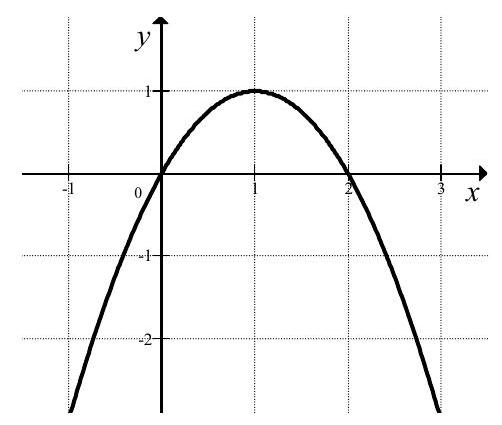
\includegraphics[max width=\textwidth, center]{2025_02_07_261058dfc2ab779a027ag-07}
\end{itemize}

\section*{II sposób}
Wyznaczamy postać kanoniczną trójmianu kwadratowego $-x^{2}+2 x$ i zapisujemy nierówność w postaci równoważnej, np.

$$
-(x-1)^{2}+1>0 .
$$

Stąd

$$
-\left((x-1)^{2}-1\right)>0 .
$$

Następnie przekształcamy nierówność do postaci równoważnej, korzystając z własności wartości bezwzględnej

$$
\begin{gathered}
(x-1)^{2}<1 \\
|x-1|<1 .
\end{gathered}
$$

\section*{Realizacja drugiego etapu}
Podajemy zbiór rozwiązań nierówności: $(0,2)$ lub $x \in(0,2)$.

\section*{Schemat punktowania}
\section*{Zdający otrzymuje}
\begin{itemize}
  \item zrealizuje pierwszy etap rozwiązania, tzn. ustali pierwiastki trójmianu kwadratowego i na tym poprzestanie lub błędnie zapisze zbiór rozwiązań nierówności, np.:
  \item obliczy lub poda pierwiastki trójmianu kwadratowego $x_{1}=0, x_{2}=2$ i na tym zakończy lub błędnie zapisze zbiór rozwiązań nierówności,
  \item zaznaczy na wykresie miejsca zerowe funkcji $f(x)=-x^{2}+2 x$ i na tym zakończy lub błędnie zapisze zbiór rozwiązań nierówności,
  \item zapisze nierówność $|x-1|<1$ i na tym zakończy lub błędnie zapisze zbiór rozwiązań nierówności\\
albo
  \item przy realizacji pierwszego etapu rozwiązania popełni błąd (ten sam błąd popełniony wielokrotnie traktuje się jak jeden błąd), ale otrzyma dwa różne pierwiastki, i konsekwentnie rozwiąże nierówność, np.:
  \item popełni błędy przy wyznaczaniu pierwiastków trójmianu kwadratowego i konsekwentnie rozwiąże nierówność,
  \item błędnie zapisze równania wynikające ze wzorów Viète’a, np. $x_{1}+x_{2}=-2$ i konsekwentnie rozwiąże nierówność,
  \item błędnie zapisze nierówność, np. $|x-1|>1$ i konsekwentnie ją rozwiąże.
\end{itemize}

\section*{Zdający otrzymuje}
gdy:

\begin{itemize}
  \item poda zbiór rozwiązań nierówności: $(0,2)$ lub $x \in(0,2)$, lub $x>0$ i $x<2$\\
albo
  \item sporządzi poprawną ilustrację geometryczną (oś liczbowa, wykres) i zapisze zbiór rozwiązań nierówności w postaci: $x>0, x<2$,\\
albo
  \item poda zbiór rozwiązań nierówności w postaci graficznej z poprawnie zaznaczonymi końcami przedziałów.\\
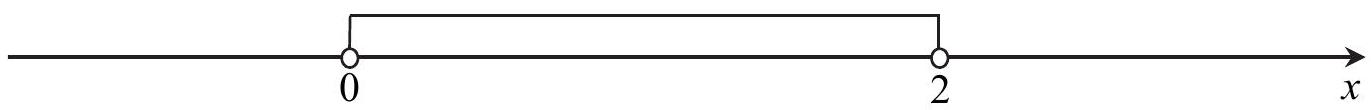
\includegraphics[max width=\textwidth, center]{2025_02_07_261058dfc2ab779a027ag-08}
\end{itemize}

\section*{Kryteria uwzględniające specyficzne trudności w uczeniu się matematyki}
Akceptujemy zapis przedziału nieuwzględniający porządku liczb na osi liczbowej, np. $(2,0)$.

\section*{Uwagi:}
\begin{enumerate}
  \item Jeżeli zdający dzieli obie strony nierówności przez $x-2$ lub przez $x$, bez stosownego założenia, to otrzymuje $\mathbf{0}$ punktów.
  \item Jeżeli zdający dzieli obie strony nierówności przez $x-2$, rozważając przy tym dwa przypadki $x>2$ i $x<2$, rozwiąże nierówność w każdym z tych przypadków oraz wyznaczy poprawny zbiór rozwiązań nierówności, to otrzymuje 2 punkty.
\end{enumerate}

Zadanie 28. (0-2)

\begin{center}
\begin{tabular}{|l|l|}
\hline
\begin{tabular}{l}
I. Wykorzystanie \\
i tworzenie informacji \\
\end{tabular} & \begin{tabular}{l}
3. Równania i nierówności. Zdający korzysta $z$ własności \\
iloczynu przy rozwiązywaniu równań typu $x(x+1)(x-7)=0$ \\
(3.7). \\
\end{tabular} \\
\hline
\end{tabular}
\end{center}

\section*{Przykładowe rozwiązanie}
Lewa strona równania jest iloczynem dwóch czynników $4-x$ oraz $x^{2}+2 x-15$. Zatem iloczyn ten jest równy 0 , gdy co najmniej jeden z tych czynników jest równy 0 , czyli

$$
4-x=0 \text { lub } x^{2}+2 x-15=0 .
$$

Rozwiązaniem równania $4-x=0$ jest $x=4$.\\
Rozwiązania równania $x^{2}+2 x-15=0$ możemy wyznaczyć, korzystając:

\begin{itemize}
  \item ze wzorów na pierwiastki trójmianu kwadratowego:
\end{itemize}

$$
\Delta=2^{2}-4 \cdot 1 \cdot(-15)=64=8^{2}, x_{1}=\frac{-2-8}{2}=-5, x_{2}=\frac{-2+8}{2}=3
$$

albo

\begin{itemize}
  \item ze wzorów Viète'a:
\end{itemize}

$$
x_{1}+x_{2}=-2 \text { oraz } x_{1} \cdot x_{2}=-15 \text { i stąd } x_{1}=-5, x_{2}=3,
$$

albo

\begin{itemize}
  \item z postaci iloczynowej trójmianu $x^{2}+2 x-15$ $(x+5)(x-3)=0$, stąd $x_{1}=-5, x_{2}=3$,\\
albo
  \item z własności wartości bezwzględnej, przekształcając najpierw równanie do postaci równoważnej $|x+1|=4$, skąd $x+1=4$ lub $x+1=-4$, czyli $x=3$ lub $x=-5$.
\end{itemize}

Zatem wszystkie rozwiązania równania to: $x=4$ lub $x=-5$, lub $x=3$.

\section*{Schemat punktowania}
\section*{Zdający otrzymuje}
1 p. gdy:

\begin{itemize}
  \item zapisze dwa równania: $4-x=0$ i $x^{2}+2 x-15=0$ (wystarczy, że z rozwiązania wynika, że zdający wyznacza pierwiastki każdego z wielomianów: $4-x, x^{2}+2 x-15$ )\\
albo
  \item zapisze rozwiązanie $x=4$,\\
albo
  \item obliczy co najmniej jeden pierwiastek trójmianu $x^{2}+2 x-15: x=-5, x=3$,\\
albo
  \item wyznaczy jeden z pierwiastków wielomianu $-x^{3}+2 x^{2}+23 x-60$\\
i na tym zakończy lub dalej popełnia błędy.
\end{itemize}

\begin{verbatim}
Zdający otrzymuje
2 p.
gdy wyznaczy bezbłędnie wszystkie rozwiązania równania: $x=-5, x=3, x=4$.
\end{verbatim}

\section*{Uwagi.}
\begin{enumerate}
  \item Jeżeli zdający obliczy trzy pierwiastki, ale w odpowiedzi końcowej podaje tylko dwa, to otrzymuje 1 punkt.
  \item Jeżeli zdający dzieli obie strony równania bez stosownego założenia przez $x-4$ lub przez drugi czynnik i oblicza pierwiastki (lub pierwiastek) dla pozostałej części, to otrzymuje 0 punktów.
\end{enumerate}

\section*{Zadanie 29. (0-2)}
V. Rozumowanie i argumentacja.\\
7. Planimetria. Zdający rozpoznaje trójkąty podobne i wykorzystuje (także w kontekstach praktycznych) cechy podobieństwa trójkątów (7.3).

\section*{Przykładowe rozwiązania}
I sposób\\
Niech $|\Varangle A C B|=\alpha$.\\
Ponieważ $|\Varangle C A B|=90^{\circ}$, więc $|\Varangle A B C|=90^{\circ}-\alpha$.\\
W $\triangle C D E:|\Varangle D E C|=90^{\circ}$, więc $|\Varangle C D E|=90^{\circ}-\alpha$.\\
Trójkąt $C D E$ jest prostokątny oraz $|\Varangle D E C|=90^{\circ}$, więc $|\Varangle C D E|=90^{\circ}-\alpha$.\\
Podobnie trójkąt $B F G$ jest prostokątny i $|\Varangle F G B|=90^{\circ}$, więc $|\Varangle B F G|=\alpha$.\\
Ponieważ trójkąty $C D E$ i $B F G$ mają równe kąty, więc na podstawie cechy podobieństwa $k k k$ są podobne.

\section*{II sposób}
Niech $|\Varangle A C B|=|\Varangle D C E|=\alpha$ i $|\Varangle A B C|=|\Varangle F B G|=\beta$.\\
Trójkąt $C E D$ jest podobny do trójkąta $A B C$ (cecha $k k k$ ), bo $|\Varangle A C B|=|\Varangle D C E|=\alpha$ oraz $|\Varangle C A B|=|\Varangle D E C|=90^{\circ}$.\\
Podobnie trójkąt $G B F$ jest podobny do trójkąta $A B C$, (cecha $k k k$ ), bo $|\Varangle A B C|=|\Varangle F B G|=\beta$ oraz $|\Varangle C A B|=|\Varangle F G B|=90^{\circ}$.\\
Stąd trójkąt $C E D$ jest podobny do trójkąta $F B G$ (z przechodniości relacji podobieństwa).

\section*{Schemat punktowania}
Zdający otrzymuje 1 p. gdy

\begin{itemize}
  \item wskaże w dwóch trójkątach spośród trójkątów $C B A, C D E$ i $F B G$ jedną parę równych kątów ostrych i na tym zakończy lub dalej popełni błędy, przy czym kąt przy wierzchołku $B$ musi być wskazany dwukrotnie, jako kąt w obu trójkątach $C B A$ i $F B G$, np. zdający zapisze $|\Varangle F B G|=|\Varangle C B A|$ lub stwierdzi, że jest to wspólny kąt trójkątów $C B A$ i $F B G$ (analogicznie z kątem przy wierzchołku $C$ w trójkątach $C B A$ i $C D E$ )\\
albo
  \item zapisze, że trójkąt $C B A$ jest podobny do trójkąta $F B G$ i do trójkąta $C D E$ i stąd wywnioskuje, że trójkąt $C D E$ jest podobny do trójkąta $F B G$, ale nie wskaże żadnej pary równych kątów ostrych w tych trójkątach i na tym zakończy lub dalej popełnia błędy.\\
Zdający otrzymuje
\end{itemize}

gdy przeprowadzi pełne rozumowanie.

Uwagi:

\begin{enumerate}
  \item Jeżeli zdający przyjmie konkretne miary kątów, to otrzymuje $\mathbf{0}$ punktów.
  \item Jeżeli zdający przyjmie błędne zależności między kątami, to otrzymuje $\mathbf{0}$ punktów.
\end{enumerate}

Zadanie 30. (0-2)\\
V. Rozumowanie i argumentacja.\\
2. Wyrażenia algebraiczne. Zdający używa wzorów skróconego mnożenia na $(a \pm b)^{2}$ oraz $a^{2}-b^{2}$ (2.1).

\section*{Przykładowe rozwiązanie}
Rozważmy wyraz $a_{n}=2 n^{2}+2 n$.\\
Wyraz $a_{n+1}$ można zapisać, jako

$$
a_{n+1}=2(n+1)^{2}+2(n+1)=2 n^{2}+6 n+4 .
$$

Wtedy

$$
a_{n}+a_{n+1}=2 n^{2}+2 n+2 n^{2}+6 n+4=4 n^{2}+8 n+4 .
$$

Zatem

$$
a_{n}+a_{n+1}=(2 n+2)^{2} .
$$

Liczba $2 n+2$ jest naturalna. To kończy dowód.

\section*{Schemat punktowania}
Zdający otrzymuje\\
gdy poprawnie zapisze sumę dwóch kolejnych wyrazów tego ciągu, np .

$$
a_{n}+a_{n+1}=2 n^{2}+2 n+2(n+1)^{2}+2(n+1)
$$

i na tym zakończy lub dalej popełnia błędy.

\section*{Zdający otrzymuje}
2 p.\\
gdy przeprowadzi pełne rozumowanie.\\
Uwaga:\\
Jeżeli zdający sprawdzi prawdziwość tezy tylko dla konkretnych wartości $n$, to otrzymuje 0 punktów.

Zadanie 31. (0-2)

\begin{center}
\begin{tabular}{|l|l|}
\hline
 & \begin{tabular}{l}
1. Liczby rzeczywiste. Zdający wykorzystuje definicję logarytmu \\
i stosuje w obliczeniach wzory na logarytm iloczynu, logarytm \\
ilorazu i logarytm potęgi o wykładniku naturalnym oraz \\
\end{tabular} \\
matematyczne. & \begin{tabular}{l}
wykorzystuje podstawowe własności potęg - również \\
w zagadnieniach związanych z innymi dziedzinami wiedzy, \\
np. fizyką, chemią, informatyką (1.6, 1.5). \\
\end{tabular} \\
\hline
\end{tabular}
\end{center}

\section*{Przykładowe rozwiązania}
\section*{I sposób}
Zapisujemy równanie

$$
6,2=\log \frac{A}{10^{-4}}
$$

Korzystamy z definicji logarytmu

$$
10^{6,2}=\frac{A}{10^{-4}}
$$

Stąd

$$
\begin{gathered}
A=10^{6,2} \cdot 10^{-4}, \\
A=10^{2,2} .
\end{gathered}
$$

Stwierdzamy, że $10^{2,2}>10^{2}=100$, gdyż funkcja wykładnicza $y=10^{x}$ jest rosnąca. Oznacza to, że $A>100 \mathrm{~cm}$.

\section*{II sposób}
Zapisujemy równanie

$$
6,2=\log \frac{A}{10^{-4}}
$$

To równanie jest równoważne kolejno równaniom

$$
\begin{gathered}
6,2=\log \left(10^{4} A\right), \\
6,2=\log 10^{4}+\log A, \\
6,2=4+\log A
\end{gathered}
$$

Zatem 2, $2=\log A$. Korzystamy z definicji logarytmu i otrzymujemy równość

$$
A=10^{2,2}
$$

Stwierdzamy, że $10^{2,2}>10^{2}=100$, gdyż funkcja wykładnicza $y=10^{x}$ jest rosnąca. Oznacza to, że $A>100 \mathrm{~cm}$.

\section*{Schemat punktowania}
Zdający otrzymuje 1 p. gdy

\begin{itemize}
  \item wykorzysta definicję logarytmu i przekształci równanie $6,2=\log \frac{A}{10^{-4}}$ do postaci $10^{6,2}=\frac{A}{10^{-4}}$\\
albo
  \item wykorzysta własność logarytmu i przekształci równanie $6,2=\log \frac{A}{10^{-4}}$ do postaci
\end{itemize}

$$
6,2=\log A-\log 10^{-4} \text { lub } 6,2=\log A+\log 10^{4}
$$

i na tym zakończy lub dalej popełnia błędy.\\
gdy zapisze, że $A=10^{2,2}$ i stwierdzi, że amplituda tego trzęsienia ziemi była większa od 100 cm .\\
Zdający otrzymuje\\
2 p.\\
Uwagi:

\begin{enumerate}
  \item Jeżeli zdający błędnie interpretuje treść zadania, w szczególności stosuje niepoprawne podstawienie do wzoru, to otrzymuje 0 punktów.
  \item Jeżeli zdający nie obliczy amplitudy, ale uzasadni, że amplituda jest większa od 100 cm , to otrzymuje 1 punkt.
  \item Jeżeli zdający nie obliczy amplitudy tylko zapisze bez uzasadnienia, że amplituda jest większa od 100 cm , to otrzymuje $\mathbf{0}$ punktów.
\end{enumerate}

Zadanie 32. (0-4)\\
IV. Użycie i tworzenie strategii.

SP9. Wielokąty, koła, okręgi. Zdający stosuje twierdzenie o sumie kątów trójkąta (SP9.3).\\
G7. Równania. Zdający rozwiązuje równania stopnia pierwszego z jedną niewiadomą (G7.3).

\section*{Przykładowe rozwiązania}
I sposób\\
Niech $\alpha$ oznacza najmniejszy kąt trójkąta. Zatem pozostałe dwa kąty tego trójkąta równe są $\alpha+50^{\circ}$ oraz $3 \alpha$. Suma kątów trójkąta jest równa $180^{\circ}$, więc

$$
\begin{gathered}
\alpha+3 \alpha+\alpha+50^{\circ}=180^{\circ}, \\
5 \alpha=130^{\circ} \\
\alpha=26^{\circ} .
\end{gathered}
$$

Stąd $\alpha+50^{\circ}=76^{\circ}$ oraz $3 \alpha=78^{\circ}$.\\
II sposób\\
Niech $\alpha$ oznacza największy kąt trójkąta. Zatem pozostałe dwa kąty tego trójkąta równe są $\frac{\alpha}{3}+50^{\circ}$ oraz $\frac{\alpha}{3}$. Suma kątów trójkąta jest równa $180^{\circ}$, więc

$$
\begin{gathered}
\frac{\alpha}{3}+\frac{\alpha}{3}+50^{\circ}+\alpha=180^{\circ} \\
5 \alpha=390^{\circ} \\
\alpha=78^{\circ}
\end{gathered}
$$

Stąd $\frac{\alpha}{3}=26^{\circ}$ oraz $\frac{\alpha}{3}+50^{\circ}=76^{\circ}$.

\section*{III sposób}
Niech $\alpha$ oznacza ten kąt trójkąta, który nie jest ani największy, ani najmniejszy. Zatem pozostałe dwa kąty tego trójkąta równe są $\alpha-50^{\circ}$ oraz $3\left(\alpha-50^{\circ}\right)$. Suma kątów trójkąta jest równa $180^{\circ}$, więc

$$
\begin{gathered}
\alpha-50^{\circ}+\alpha+3\left(\alpha-50^{\circ}\right)=180^{\circ} \\
5 \alpha=380^{\circ} \\
\alpha=76^{\circ}
\end{gathered}
$$

Stąd $\alpha-50^{\circ}=26^{\circ}$ oraz $3\left(\alpha-50^{\circ}\right)=78^{\circ}$.

\section*{Schemat punktowania}
Rozwiązanie, w którym postęp jest niewielki, ale konieczny na drodze do pełnego rozwiązania. Zdający zapisze:

\begin{itemize}
  \item kąty trójkąta w zależności od jednego kąta, np.:
\end{itemize}

$$
\alpha, \alpha+50^{\circ}, 3 \alpha \quad \text { lub } \quad \frac{\alpha}{3}, \frac{\alpha}{3}+50^{\circ}, \alpha, \text { lub } \quad \alpha-50^{\circ}, \alpha, 3\left(\alpha-50^{\circ}\right)
$$

albo

\begin{itemize}
  \item układ dwóch równań, np.
\end{itemize}

$$
\left\{\begin{array}{l}
\alpha+\alpha+50^{\circ}+\beta=180^{\circ} \\
\beta=3 \alpha
\end{array}\right.
$$

albo

\begin{itemize}
  \item układ trzech równań, np.
\end{itemize}

$$
\left\{\begin{array}{l}
\alpha+\beta+\gamma=180^{\circ} \\
\gamma=3 \alpha \\
\beta=\alpha+50^{\circ}
\end{array}\right.
$$

i na tym zakończy lub dalej popełnia błędy.\\
Rozwiązanie, w którym jest istotny postęp\\
Zdający zapisze równanie z jedną niewiadomą, np.:

$$
\alpha+3 \alpha+\alpha+50^{\circ}=180^{\circ} \text { lub } \frac{\alpha}{3}+\frac{\alpha}{3}+50^{\circ}+\alpha=180^{\circ}, \text { lub } \alpha-50^{\circ}+\alpha+3\left(\alpha-50^{\circ}\right)=180^{\circ}
$$

i na tym zakończy lub dalej popełnia błędy.\\
Pokonanie zasadniczych trudności zadania. 3 p.\\
Zdający obliczy jeden z kątów trójkąta, np.: $\alpha=26^{\circ}$ lub $\alpha=78^{\circ}$, lub $\alpha=76^{\circ}$ i na tym zakończy lub dalej popełnia błędy.\\
Rozwiązanie petne.\\
Zdający obliczy wszystkie kąty trójkąta.

\section*{Uwagi:}
\begin{enumerate}
  \item Jeżeli zdający tylko poda kąty ( $26^{\circ}, 76^{\circ}, 78^{\circ}$ ), to otrzymuje $\mathbf{1}$ punkt.
  \item Jeżeli zdający tylko poda kąty i sprawdzi wszystkie warunki zadania, to otrzymuje $\mathbf{2}$ punkty.
\end{enumerate}

Zadanie 33. (0-5)

\begin{center}
\begin{tabular}{|l|l|}
\hline
\begin{tabular}{l}
IV. Użycie i tworzenie \\
strategii. \\
\end{tabular} & \begin{tabular}{l}
9. Stereometria. Zdający stosuje trygonometrię do obliczeń \\
długości odcinków, miar kątów, pól powierzchni i objętości \\
(9.6). \\
G10. Figury płaskie. Zdający stosuje twierdzenie Pitagorasa \\
(G10.7). \\
\end{tabular} \\
\hline
\end{tabular}
\end{center}

\section*{Przykładowe rozwiązanie}
Wprowadzamy oznaczenia jak na rysunku.\\
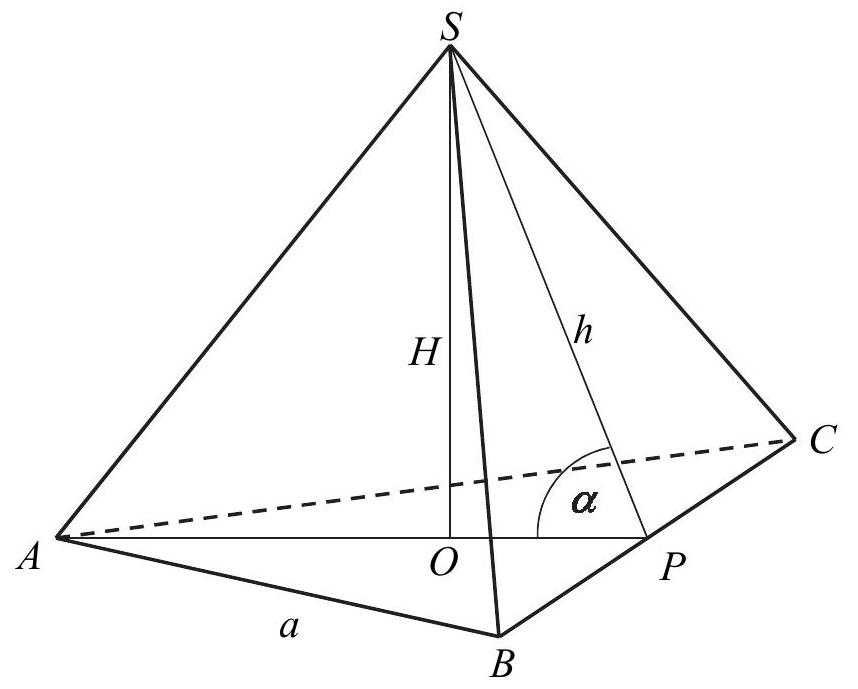
\includegraphics[max width=\textwidth, center]{2025_02_07_261058dfc2ab779a027ag-15}

Ponieważ wysokość tego ostrosłupa jest równa wysokości jego podstawy, to $H=\frac{a \sqrt{3}}{2}$. Objętość ostrosłupa jest równa 27, więc otrzymujemy równanie

$$
\frac{1}{3} \cdot \frac{a^{2} \sqrt{3}}{4} \cdot \frac{a \sqrt{3}}{2}=27
$$

skąd otrzymujemy $a=6$.\\
Wysokość ostrosłupa jest równa

$$
H=\frac{6 \sqrt{3}}{2}=3 \sqrt{3} .
$$

Punkt $O$ jest środkiem okręgu opisanego na trójkącie równobocznym $A B C$, zatem długość odcinka $P O$ stanowi $\frac{1}{3}$ wysokości trójkąta $A B C$, czyli

$$
|O P|=\frac{1}{3} H=\frac{1}{3} \cdot 3 \sqrt{3}=\sqrt{3} .
$$

Z twierdzenia Pitagorasa zastosowanego dla trójkąta $P O S$ otrzymujemy

$$
\begin{gathered}
h^{2}=|O P|^{2}+H^{2}, \\
h^{2}=(\sqrt{3})^{2}+(3 \sqrt{3})^{2}, \\
h^{2}=30 .
\end{gathered}
$$

Stąd

$$
h=\sqrt{30} .
$$

Pole powierzchni bocznej ostrosłupa jest zatem równe

$$
P_{b}=3 \cdot \frac{1}{2} a h=3 \cdot \frac{1}{2} \cdot 6 \sqrt{30}=9 \sqrt{30} .
$$

Cosinus kąta nachylenia wysokości ściany bocznej do płaszczyzny podstawy jest równy

$$
\cos \alpha=\frac{|O P|}{h}=\frac{\sqrt{3}}{\sqrt{30}}=\frac{\sqrt{10}}{10} .
$$

\section*{Schemat punktowania}
\section*{Rozwiązanie, w którym postęp jest niewielki, ale konieczny na drodze}
 do pełnego rozwiązania. 1 p. Zdający:\begin{itemize}
  \item zapisze równanie, z którego można obliczyć długość krawędzi podstawy ostrosłupa:
\end{itemize}

$$
\frac{1}{3} \cdot \frac{a^{2} \sqrt{3}}{4} \cdot \frac{a \sqrt{3}}{2}=27
$$

albo

\begin{itemize}
  \item zapisze równanie, z którego można obliczyć wysokość ostrosłupa:
\end{itemize}

$$
\frac{1}{3} \cdot \frac{\left(\frac{2 H}{\sqrt{3}}\right)^{2} \sqrt{3}}{4} \cdot H=27
$$

i na tym zakończy lub dalej popełnia błędy.\\
Rozwiązanie, w którym jest istotny postęp\\
Zdający obliczy długość krawędzi podstawy ostrosłupa $a=6$ lub wysokość ostrosłupa $H=3 \sqrt{3}$ i na tym zakończy lub dalej popełnia błędy.\\
Uwaga:\\
Zdający może obliczyć od razu tangens kąta nachylenia wysokości ściany bocznej do płaszczyzny podstawy ostrosłupa:

$$
\operatorname{tg} \alpha=\frac{H}{\frac{1}{3} H}=3
$$

a następnie obliczyć szukaną wartość cosinusa tego kąta:

$$
\cos \alpha=\frac{\sqrt{10}}{10}
$$

Otrzymuje wtedy 2 punkty.\\
Pokonanie zasadniczych trudności zadania\\
Zdający obliczy

\begin{itemize}
  \item wysokość ściany bocznej ostrosłupa: $\sqrt{30}$\\
albo
  \item długość krawędzi bocznej ostrosłupa: $\sqrt{39}$\\
i na tym zakończy lub dalej popełnia błędy.
\end{itemize}

\section*{Rozwiązanie prawie pełne}
\section*{Zdający obliczy:}
\begin{itemize}
  \item pole powierzchni bocznej ostrosłupa $A B C S: 9 \sqrt{30}$\\
albo
  \item cosinus kąta nachylenia wysokości ściany bocznej do płaszczyzny podstawy:
\end{itemize}

$$
\cos \alpha=\frac{\sqrt{10}}{10}
$$

i na tym zakończy lub dalej popełnia błędy.

\section*{Rozwiązanie pełne}
Zdający obliczy pole powierzchni bocznej ostrostupa $A B C S$ : $9 \sqrt{30}$ i cosinus kąta nachylenia wysokości ściany bocznej do płaszczyzny podstawy: $\cos \alpha=\frac{\sqrt{10}}{10}$.

\section*{Uwagi:}
\begin{enumerate}
  \item Jeżeli zdający rozważa inną bryłę niż podana w zadaniu, to za całe rozwiązanie otrzymuje 0 punktów.
  \item Jeżeli zdający popełni błąd merytoryczny np. w zastosowaniu twierdzenia Pitagorasa przy obliczaniu wysokości ściany bocznej lub w interpretacji własności trójkąta równobocznego, to otrzymuje za całe rozwiązanie otrzymuje co najwyżej 2 punkty.
  \item Akceptujemy poprawne przybliżenia dziesiętne liczb rzeczywistych.
\end{enumerate}

Zadanie 34. (0-4)\\
III. Modelowanie matematyczne.\\
10. Elementy statystyki opisowej. Teoria prawdopodobieństwa i kombinatoryka. Zdający oblicza prawdopodobieństwa w prostych sytuacjach, stosując klasyczną definicję prawdopodobieństwa (10.3).

\section*{Przykładowe rozwiązania}
\section*{I sposób}
Zdarzeniem elementarnym jest uporządkowana para $(x, y)$ dwóch różnych liczb ze zbioru $\{10,11,12, \ldots, 99\}$, który zawiera 90 liczb. Liczba wszystkich zdarzeń elementarnych jest równa $|\Omega|=90 \cdot 89$. Wszystkie zdarzenia elementarne są równo prawdopodobne. Mamy więc do czynienia z modelem klasycznym.\\
Niech $A$ oznacza zdarzenie polegające na tym, że suma wylosowanych liczb jest 30 .\\
Zatem zdarzeniu $A$ sprzyjają następujące zdarzenia elementarne:\\
$(10,20),(11,19),(12,18),(13,17),(14,16),(16,14),(17,13),(18,12),(19,11),(20,10)$.\\
Ich liczba jest równa $|A|=10$.\\
Prawdopodobieństwo zdarzenia $A$ jest równe

$$
P(A)=\frac{|A|}{|\Omega|}=\frac{10}{90 \cdot 89}=\frac{1}{9 \cdot 89}=\frac{1}{801} .
$$

Odpowiedź: Prawdopodobieństwo zdarzenia polegającego na tym, że wylosujemy dwie różne liczby dwucyfrowe, których suma jest równa 30 jest równe $\frac{1}{801}$.

\section*{II sposób}
Zdarzeniem elementarnym jest zbiór dwuelementowy $\{x, y\}$ dwóch różnych liczb ze zbioru $\{10,11,12, \ldots, 99\}$, który zawiera 90 liczb. Liczba wszystkich zdarzeń elementarnych jest równa $|\Omega|=\binom{90}{2}=\frac{90!}{88!\cdot 2!}=\frac{90 \cdot 89}{2}=4005$. Wszystkie zdarzenia elementarne są równo prawdopodobne. Mamy więc do czynienia z modelem klasycznym.\\
Niech $A$ oznacza zdarzenie polegajace na tym, że suma wylosowanych liczb jest 30. Zatem zdarzeniu $A$ sprzyjają następujące zdarzenia elementarne:

$$
\{10,20\},\{11,19\},\{12,18\},\{13,17\},\{14,16\} .
$$

Ich liczba jest równa $|A|=5$.\\
Prawdopodobieństwo zdarzenia $A$ jest równe

$$
P(A)=\frac{|A|}{|\Omega|}=\frac{5}{45 \cdot 89}=\frac{1}{9 \cdot 89}=\frac{1}{801} .
$$

Odpowiedź: Prawdopodobieństwo zdarzenia polegającego na tym, że wylosujemy dwie różne liczby dwucyfrowe, których suma jest równa 30 jest równe $\frac{1}{801}$.

\section*{III sposób}
Rysujemy drzewo z uwzględnieniem wszystkich gałęzi, które prowadzą do sytuacji sprzyjających zdarzeniu $A$ (polegającemu na tym, że suma wylosowanych liczb będzie równa 30).\\
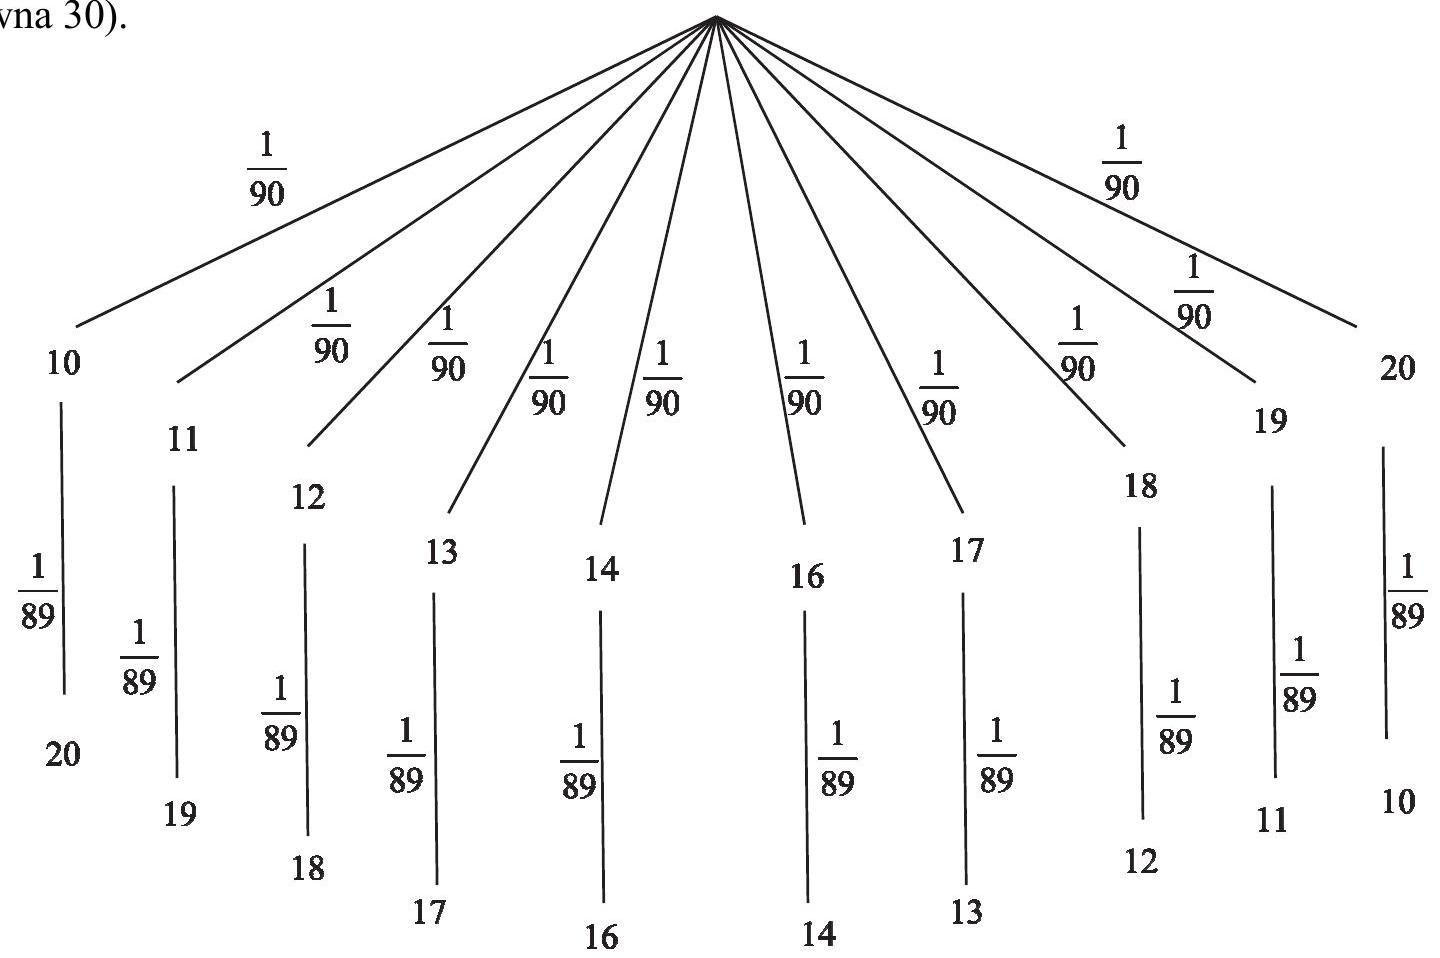
\includegraphics[max width=\textwidth, center]{2025_02_07_261058dfc2ab779a027ag-18}

Prawdopodobieństwo zdarzenia $A$ jest równe

$$
P(A)=10 \cdot \frac{1}{90} \cdot \frac{1}{89}=\frac{1}{9 \cdot 89}=\frac{1}{801} .
$$

Odpowiedź: Prawdopodobieństwo zdarzenia polegającego na tym, że wylosujemy dwie różne liczby dwucyfrowe, których suma jest równa 30 jest równe $\frac{1}{801}$.

\section*{Schemat punktowania}
\section*{Rozwiązanie, w którym postęp jest niewielki, ale konieczny na drodze do pełnego rozwiązania}
Zdający

\begin{itemize}
  \item zapisze, że wszystkich liczb naturalnych dwucyfrowych jest 90\\
albo
  \item wypisze zdarzenia elementarne sprzyjające zdarzeniu $A$ :
\end{itemize}

$$
\begin{gathered}
(10,20),(11,19),(12,18),(13,17),(14,16),(16,14), \\
(17,13),(18,12),(19,11),(20,10) \\
\text { lub }\{10,20\},\{11,19\},\{12,18\},\{13,17\},\{14,16\},
\end{gathered}
$$

albo

\begin{itemize}
  \item zapisze, że $|A|=10$ lub $|A|=5$,\\
albo
  \item narysuje drzewo ilustrujące przebieg doświadczenia (na rysunku muszą wystąpić wszystkie istotne gałęzie)\\
i na tym zakończy lub dalej popełni błędy.\\
Rozwiązanie, w którym jest istotny postęp 2 p.\\
Zdający
  \item zapisze, że wszystkich liczb naturalnych dwucyfrowych jest 90 oraz wypisze wszystkie zdarzenia elementarne sprzyjające zdarzeniu $A$ :
\end{itemize}

$$
\begin{gathered}
(10,20),(11,19),(12,18),(13,17),(14,16),(16,14), \\
(17,13),(18,12),(19,11),(20,10) \\
\text { lub }\{10,20\},\{11,19\},\{12,18\},\{13,17\},\{14,16\}
\end{gathered}
$$

albo

\begin{itemize}
  \item zapisze, że wszystkich liczb naturalnych dwucyfrowych jest 90 oraz zapisze, że $|A|=10$ lub $|A|=5$,\\
albo
  \item obliczy liczbę wszystkich zdarzeń elementarnych: $|\Omega|=90 \cdot 89$ lub $|\Omega|=\binom{90}{2}$, lub
\end{itemize}

$$
|\Omega|=\frac{90 \cdot 89}{2}, \operatorname{lub}|\Omega|=4005,
$$

albo

\begin{itemize}
  \item narysuje drzewo ze wszystkimi istotnymi gałęziami i zapisze prawdopodobieństwa na wszystkich istotnych odcinkach jednego $z$ etapów lub na jednej z istotnych gałęzi i na tym zakończy lub dalej popełni błędy.
\end{itemize}

\section*{Zdający}
\begin{itemize}
  \item obliczy liczbę wszystkich zdarzeń elementarnych: $|\Omega|=90.89$ oraz zapisze, że $|A|=10$ albo
  \item obliczy liczbę wszystkich zdarzeń elementarnych: $|\Omega|=\binom{90}{2}$ lub $|\Omega|=\frac{90 \cdot 89}{2}$, lub
\end{itemize}

$$
|\Omega|=4005 \text { oraz zapisze, że }|A|=5,
$$

albo

\begin{itemize}
  \item obliczy prawdopodobieństwo wzdłuż jednej istotnej gałęzi narysowanego drzewa:
\end{itemize}

$$
\frac{1}{90} \cdot \frac{1}{89}
$$

i na tym zakończy lub dalej popełni błędy.

\section*{Rozwiązanie pełne 4 p.}
Zdający obliczy prawdopodobieństwo zdarzenia $A: P(A)=\frac{|A|}{|\Omega|}=\frac{1}{801}$.

\section*{Uwagi:}
\begin{enumerate}
  \item Jeżeli zdający poprawnie wyznaczy moc zbioru wszystkich zdarzeń elementarnych, ale przy wyznaczaniu liczby zdarzeń sprzyjających zdarzeniu $A$ pominie jedno zdarzenie elementarne lub popełni błąd przy zliczaniu poprawnie wypisanych zdarzeń elementarnych sprzyjających zdarzeniu $A$ i konsekwentnie rozwiąże zadanie do końca, to otrzymuje 3 punkty.
  \item Jeżeli zdający błędnie zapisze, że wszystkich liczb dwucyfrowych jest 89 i konsekwentnie rozwiąże zadanie do końca, to otrzymuje 3 punkty.
  \item Jeżeli w rozwiązaniu występuje sprzeczność modeli probabilistycznych, to zdający może otrzymać, co najwyżej 2 punkty.
  \item Akceptujemy sytuacje, gdy zdający zamiast wypisywania zdarzeń elementarnych sprzyjających zdarzeniu $A$ zapisze następujące sumy $10+20,11+19,12+18,13+17$, $14+16,16+14,17+13,18+12,19+11,20+10$ (lub tylko $10+20,11+19,12+18$, $13+17,14+16)$.
  \item Jeżeli zdający zapisze, że wszystkich liczb naturalnych dwucyfrowych jest 90, ale przy wypisywaniu zdarzeń elementarnych sprzyjających zdarzeniu $A$, zapisuje sumę $15+15$ i na tym zakończy to otrzymuje 1 punkt.
  \item Jeżeli zdający bez żadnych obliczeń poda tylko wynik, np. $\frac{1}{801}$, to otrzymuje za całe rozwiązanie 1 punkt.
\end{enumerate}

\end{document}